\documentclass[
	% -- opções da classe memoir --
	12pt,				% tamanho da fonte
	% openright,			% capítulos começam em pág ímpar (insere página vazia caso preciso)
    oneside,			% para impressão somente frente. Oposto a twoside (frente e verso)
	a4paper,			% tamanho do papel. 
	% -- opções da classe abntex2 --
	%chapter=TITLE,		% títulos de capítulos convertidos em letras maiúsculas
	%section=TITLE,		% títulos de seções convertidos em letras maiúsculas
	%subsection=TITLE,	% títulos de subseções convertidos em letras maiúsculas
	%subsubsection=TITLE,% títulos de subsubseções convertidos em letras maiúsculas
	% -- opções do pacote babel --
	english,			% idioma adicional para hifenização
	french,				% idioma adicional para hifenização
	spanish,			% idioma adicional para hifenização
	brazil,				% o último idioma é o principal do documento
	]{abntex2}


% ---
% PACOTES
% ---

% ---
% Pacotes fundamentais 
% ---
\usepackage{cmap}				% Mapear caracteres especiais no PDF
\usepackage{lmodern}			% Usa a fonte Latin Modern
\usepackage[T1]{fontenc}		% Selecao de codigos de fonte.
\usepackage[utf8]{inputenc}		% Codificacao do documento (conversão automática dos acentos)
\usepackage{indentfirst}		% Indenta o primeiro parágrafo de cada seção.
\usepackage{color}				% Controle das cores
\usepackage{graphicx}			% Inclusão de gráficos
\usepackage{amsmath}
\usepackage{rotating}
% ---

% ---
% Pacotes adicionais, usados no anexo do modelo de folha de identificação
% ---
\usepackage{multicol}
\usepackage{multirow}
% ---
	
% ---
% Pacotes adicionais, usados apenas no âmbito do Modelo Canônico do abnteX2
% ---
\usepackage{lipsum}				% para geração de dummy text
% ---

% ---
% Pacotes de citações
% ---
\usepackage[brazilian,hyperpageref]{backref}	 % Paginas com as citações na bibl
\usepackage[alf]{abntex2cite}	% Citações padrão ABNT

% --- 
% CONFIGURAÇÕES DE PACOTES
% --- 

% ---
% Configurações do pacote backref
% Usado sem a opção hyperpageref de backref
\renewcommand{\backrefpagesname}{Citado na(s) página(s):~}
% Texto padrão antes do número das páginas
\renewcommand{\backref}{}
% Define os textos da citação
\renewcommand*{\backrefalt}[4]{
	\ifcase #1 %
		Nenhuma citação no texto.%
	\or
		Citado na página #2.%
	\else
		Citado #1 vezes nas páginas #2.%
	\fi}%
% ---

% ---
% Informações de dados para CAPA e FOLHA DE ROSTO
% --- PROPOSTA DE COMBATE AO FUNGO M. perniciosa, CAUSADOR DA DOENÇA VASSOURA DE BRUXA NO CACAU
\titulo{Segmentação de Placas Veiculares com técnicas de Processamento de Imagens}
\autor{Douglas Diniz Landim}
\local{São José dos Campos}
\data{2019}
\instituicao{%
  Universidade Federal de São Paulo -- UNIFESP
  \par
   Instituto de Ciência e Tecnologia -- ICT
  \par
  Ciência da Computação}
% O preambulo deve conter o tipo do trabalho, o objetivo, 
% o nome da instituição e a área de concentração 
\preambulo{Aplicação de conceitos teóricos da disciplina de Processamento de Imagens. Professora Regina Célia Coelho.}
% ---

% ---
% Configurações de aparência do PDF final

% alterando o aspecto da cor azul
\definecolor{blue}{RGB}{41,5,195}

% informações do PDF
\makeatletter
\hypersetup{
     	%pagebackref=true,
		pdftitle={\@title}, 
		pdfauthor={\@author},
    	pdfsubject={\imprimirpreambulo},
	    pdfcreator={LaTeX with abnTeX2},
		pdfkeywords={abnt}{latex}{abntex}{abntex2}{relatório técnico}, 
		colorlinks=true,       		% false: boxed links; true: colored links
    	linkcolor=blue,          	% color of internal links
    	citecolor=blue,        		% color of links to bibliography
    	filecolor=magenta,      		% color of file links
		urlcolor=blue,
		bookmarksdepth=4
}
\makeatother
% --- 

% --- 
% Espaçamentos entre linhas e parágrafos 
% --- 

% O tamanho do parágrafo é dado por:
\setlength{\parindent}{1.3cm}

% Controle do espaçamento entre um parágrafo e outro:
\setlength{\parskip}{0.2cm}  % tente também \onelineskip

% ---
% compila o indice
% ---
\makeindex
% ---

% ----
% Início do documento
% ----
\begin{document}

% Retira espaço extra obsoleto entre as frases.
\frenchspacing 

% ----------------------------------------------------------
% ELEMENTOS PRÉ-TEXTUAIS
% ----------------------------------------------------------
% \pretextual

% ---
% Capa
% ---
	\imprimircapa
% ---

% ---
% Folha de rosto
% (o * indica que haverá a ficha bibliográfica)
% ---
\imprimirfolhaderosto*
% ---
	


% ---
% RESUMO
% ---

% resumo na língua vernácula (obrigatório)
\begin{resumo} %% AQUI COMEÇA A PÁGINA DE RESUMO

Com a crescente automatização dos sistemas de controle e interação entre veículos que não se limitam mais apenas na fiscalização de velocidade, mas também em aplicações como controle de estacionamento, acesso de condomínios, sistema de segurança, entre outros; faz surgir a necessidade de desenvolvimento de sistemas e métodos que sejam capazes de realizar a identificação dos veículos de forma simples e eficiente. Assim, a identificação das placas veiculares pode auxiliar na tomada de dados para os mais diversos usos. Para tanto, a Utilização de técnicas de processamento de imagem, visando a extração de atributos desejados de um objeto em imagens digitais, pode ser de grande valia. Essas técnicas visam, além da identificação dos caracteres presentes em cada placa, auxiliar no pré tratamento das imagens com a possibilidade de remoção de ruídos e extração bordas. Portanto, Este trabalho objetivou a utilização e combinação de métodos de segmentação para a identificação de placas automotivas. O resultado deste trabalho produz imagens segmentadas, prontas para serem utilizadas em métodos de visão computacional que podem extrair informações semânticas das imagens. O processo de segmentação foi formado em 5 etapas: i) a imagem de uma placa veicular é tratada com remoção de ruídos através do filtro de mediana; ii) em seguida aplica-se a redução de dimensão (binarização); iii) na terceira etapa são aplicadas operações morfológicas para remoção de objetos e componentes pequenos que não correspondem às informações de interesse da placa; iv) extração dos maiores componentes conexos da imagem inferindo-se que todos serão respectivos aos caracteres de interesse à se segmentar; v) por fim na quinta etapa é extraído o gradiente morfológico dos objetos finais segmentados, aplicando por fim as métricas de avaliação de segmentação pelos métodos de Dicce e Jaccard.


% Processamento de Imagens são processamentos realizados sobre uma imagem com o objetivo de melhorar sua qualidade, extrair atributos visuais, restaurá-la entre outras possíveis melhorias a fim de melhorar a informação visual para humanos ou processar dados de cenas.

% Uma aplicação importante de processamento de imagens é na área de análise de tráfego. Hoje em dias, inúmeras câmeras monitoram ruas, avenidas e rodovias, obtendo informações úteis e relevantes sobre os automóveis. 
 
% Esse trabalho visa reproduzir um sistema de reconhecimento automático de placas a fim de estudar métricas de desempenho e aplicar os conhecimentos teóricos obtidos em aula. 

% apresentar o problema

% dizer a solução 

% apresentar a matéria


% dizer os objetivos


 \vspace{\onelineskip}
    
 \noindent
 \textbf{Palavras-chaves}: Processamento de imagens, Placa de carro, Segmentação por Otsu. Operações Morfológicas.
\end{resumo} %AQUI TERMINA A PÁGINA DE RESUMO
% ---

% ---
% inserir lista de ilustrações
% ---

\listoffigures* %% o * indica que não será incluso no sumário
\cleardoublepage %% Pula página
% ---
% ---
% ---
% ---
% inserir o sumario
% ---

\tableofcontents*

% ---

% ----------------------------------------------------------
% ELEMENTOS TEXTUAIS  (necessário para incluir número nas páginas)
% ----------------------------------------------------------
\textual


% ----------------------------------------------------------
% Introdução
% ----------------------------------------------------------
\chapter{Introdução} 


O monitoramento de ruas, avenidas e estradas é de grande importância para o gerenciamento e bom funcionamento das vias terrestres. Uma alternativa de monitoramento é a identificação veicular por meio de sua placa, o qual pode fornecer dados para diversas aplicações, como exemplo: coleta de dados para controle tráfego, gerenciamento de vagas em estacionamento, cobrança de taxas em rodovias e cumprimento dos limites de velocidade.

Atualmente o sistema utilizado pelo Detran (Departamento de Trânsito) utiliza a tecnologia OCR em um sistema de Leitura Automática de Placas \cite{ming2006fiscalizaccao}. Seguindo a tendência de automatização de processos, a utilização de imagens coletadas por radares e sistemas de vigilância aplicadas à algoritmos de detecção de padrões tem se mostrado eficiente e de baixo custo na identificação de placas de carros. 

Desta forma a utilização de métodos de processamento de imagens que possam auxiliar na remoção de ruídos e na restauração de imagens que possuam placas de carro, buscando à extração de atributos utilizáveis por algoritmos especializados em detecção de padrões, apresentam-se com grande potencial.


Portanto, este trabalho teve como objetivo desenvolver um sistema para a detecção de placas veiculares utilizando técnicas de processamento de imagem em ambiente MatLab. Todavia, o presente trabalho buscou não somente explorar funções pré definidas na linguagem, mas realizar adicionalmente a implementação das funções de filtro de ruídos por mediana, segmentação e binarização pelo método de Otsu, e operações morfológicas básicas como erosão, dilatação, abertura e fechamento, que auxiliarão no processo de identificação das placas. 




%Aqui você começa a escrever seu trabalho \cite{fulano}. Este documento e seu código-fonte são exemplos de referência de uso da classe
%\textsf{abntex2} e do pacote \textsf{abntex2cite}. O documento 
%exemplifica a elaboração de relatórios técnicos e/ou científicos produzidos
%conforme a ABNT NBR 10719:2011 \textit{Informação e documentação - Relatório
%técnico e/ou científico - Apresentação}.


% ----------------------------------------------------------
% Capitulo 2
% ----------------------------------------------------------
\chapter{Desenvolvimento}

\section{Objetivos}

\subsection{Objetivo Geral}

O objetivo geral desse trabalho foi desenvolver um sistema de segmentação de placas veiculares, a partir do uso e implementação de técnicas de processamento de imagens. 
Este trabalho entrega como resultado imagens segmentadas para aplicação de métodos de visão computacional, que por sua vez fazem identificação de padrões e reconhecimento das informações contextuais das imagens segmentadas.

\subsection{Objetivos específicos}

\begin{itemize}

\item  Realizar filtragem de ruído das imagens de placas veiculares.
\item  Binarização das imagens por Otsu.
\item  Operações Morfólogicas e tratamento da imagem binarizada para eliminação de ruído e informações irrelevantes.
\item  Isolamento das letras e números das placas por meio de obtenção de componentes conexos.
\item  Aplicação das métricas de avaliação das imagens segmentadas.

\end{itemize}

%\url{http://www.ceplac.gov.br/radar/mercado_cacau.htm}

%\url{http://www.sober.org.br/palestra/5/546.pdf}

\section{Metodologia}

O processo metodológico envolvido na realização deste projeto está apresentado na Figura \ref{fig:mat_met}. Os materiais utilizados estão representados pelo quadro amarelo; Os processos de cada etapa estão representados em azul, As técnicas/pacotes utilizados estão representados em Verde. Os materiais e processos, bem como seus respectivos pacotes e implementações serão descritos de forma mais abrangente ao longo desta secção. Todos os códigos envolvidos na implementação deste projeto podem ser encontrados no repositório do \textit{github} sob o domínio \textit{https://github.com/ddlandim/cs-unifespbr-processamentoImagens/tree/master/placa\_carro\_segmentacaos}.

\begin{figure}[!ht]
    \centering
    \includegraphics[scale=0.85]{figuras/Diagrama_met_novo.jpeg}
    \caption{Etapas para detecção dos caracteres das placas de carro.}
    \label{fig:mat_met}
\end{figure}

Ainda que com grande recorrência na literatura, trabalhos para o desenvolvimento de algoritmos segmentação e sistemas de detecção e identificação de placas automotivas esbarram, inicialmente, na disponibilidade de um base de dados consistente. Na maior parte dos casos estas imagens estão sob domínio privado e de acesso restrito, o qual leva a aquisição de uma base de dados de imagens ou a realização de captação manual das imagens. Ainda que se apresente um trabalho moroso, a busca das imagens de forma manual por meio da utilização de plataformas como o \textit{Google} ou \textit{Bing}, evita a adição de custos financeiros ao projeto. Portanto, para o presente trabalho um banco de imagens de placas automotivas foi formado por meio da captação manual de imagens disponíveis na ferramenta de busca de imagens do \textit{Google} e em pastas de imagens de trabalhos relacionados no \textit{Github}. 

As placas de identificação de veículos no Brasil são emitidas pelos Departamentos Estaduais de Trânsito (DETRANs) de cada estado e do Distrito Federal, seguindo um sistema alfanumérico comum a todo o país. A seleção dos tipos de placas consistiu na escolha no padrão vigente composto por três letras e quatro números, no formato ABC·1234, vigente desde {1990} até atualmente, seguindo a Resolução 231 de 2007 do Denatran \cite{res231}.Este modelo foi selecionado devido a falta de um padrão exato defino anteriormente a resolução 231 e a pouca abrangência do novo modelo, criado em função de um acordo entre os países do Mercosul. Assim, foram selecionadas apenas imagens do padrão de maior recorrência na frota de veículos brasileira. A Figura \ref{fig:exemplo_placa} apresenta um exemplo do tipo de placa selecionado. Buscando atender o escopo deste trabalho, optou-se por utilizar imagens compostas somente por placas, evitando necessidade de uma pré-segmentação para extrair a placa de uma imagem com o carro ou o ambiente ao redor.


%  Desde 2018 coexistem dois sistemas alfanuméricos: um com três letras e quatro números, no formato ABC·1234, vigente desde 1990 e que segue a Resolução 231 de 2007 do Denatran[1] e outro, com quatro letras e três números, no formato ABC1D23, também conhecido como "padrão Mercosul", por seguir a diretiva do bloco econômico, conforme as regras da Resolução 780 de 2019[2]. 

\begin{figure}[!ht]
    \centering
    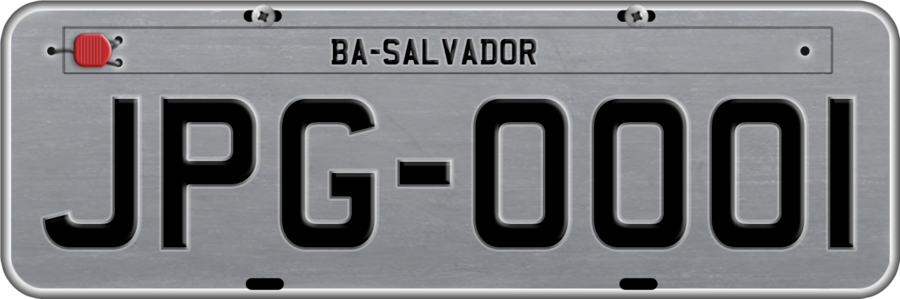
\includegraphics[scale=0.32]{figuras/placa.png}
    \caption{Exemplo de placa veicular sem ruído.}
    \label{fig:exemplo_placa}
\end{figure}

Outro fator importante a ser considerado na criação do banco de imagens de validação do algoritmo criado é a presença de ruídos nas imagens, devido a baixa resolução de câmeras de monitoramento e dos sistemas de radares. Assim, foram selecionadas não só imagens de boa qualidade, como também imagens que apresentavam ruídos, classificados em baixa, média e alta influência no processo de detecção. A Figura \ref{fig:placa_ruido} apresenta os tipos de ruídos encontrados nas placas selecionadas.

\begin{figure}[!ht]
    \centering
    \includegraphics[scale=0.25]{figuras/1.jpg}
    \caption{Exemplo de placa veicular com ruído.}
    \label{fig:placa_ruido}
\end{figure}

%( \cite{mello2009complete}, \cite{prates2014brazilian}, \cite{chang2004automatic})

A partir do banco de dados já formado, os seguintes passos foram aplicados, sendo que cada método é explanado melhor nas secções a seguir:

1 - Pré-processamento 

    - Imagens já obtidas do banco com dimensão reduzida e área da placa centralizada.
    
    - Conversão para escala de cinza.
    
2 - Processamentos 

    - Filtragem de ruido da imagem.
    
    - Segmentação e Binarização.
    
    - Filtragem de ruído e objetos pequenos com operação morfológica de abertura na imagem binarizada.
    
    - Obtenção dos 7 maiores componentes conexos e remoção dos restantes
    
    - Avaliação das métricas de Dice e Jaccard. 
    
    

\subsection{Pré-processamento}

Dimensionalidade:
Buscando reduzir a dimensionalidade das imagens selecionadas, todas as imagens foram submetidas a um processo de transformação dos valores de cor (RGB) em escala de cinzas, reduzindo de três para uma dimensão, respectivamente. Desta forma a dimensão remanescente é comumente conhecida como "intensidade", sendo esta composta por 255 níveis de intensidade, ou seja 8 bits. A conversão para escala de cinza neste processo de segmentação de placas veiculares é essencial pois o objetivo do principal do processo é a obtenção de informações referentes aos caracteres presentes na placa, e tal informação é independente da cor do caractere. 

Em fotografias digitais, uma imagem em escala de cinza é aquela em que o valor de cada pixel é uma amostra única representando apenas uma quantidade de luz, ou seja, ela carrega apenas informações de intensidade. Imagens em escala de cinza, são uma espécie de monocromático entre preto e branco (ou cinza), compostas exclusivamente por tons de cinza. O contraste varia de preto na intensidade mais fraca a branco na mais forte \cite{johnson2006}.



O recorte centralizado da imagem é necessário, pois imagens com fundo preto impactam diretamente no processo de segmentação, visto que a técnica de otsu utiliza calcula variâncias globais e locais de intensidades de pixels, e um fundo com intensidade muito próxima do objeto a ser segmentado interfere diretamente no processo.


Ter um processo de segmentação invariante à escala das imagens de entrada é um desafio pois na etapa de remoção de ruídos tanto na imagem de entrada quanto na imagem binarizada, utiliza-se elementos estruturantes com tamanhos pré-determinados, sendo assim, imagens muito pequenas em relação às imagens utilizadas na parametrização de processo de segmentação, podem sofrer com destruição de objetos principais juntamente com os ruídos.

\subsection{Remoção de ruídos}

A primeira etapa do processamento na identificação dos caracteres presentes nas placas de veículos automotivos consiste na aplicação de técnicas de remoção de ruídos, uma vez que os ruídos presentes nas imagens obtidas podem levar o classificador a resultados inconsistentes. Buscando determinar o filtro anti-ruído mais adequado para o presente trabalho, os filtros de média, mediana, passa-baixa e passa-alta foram avaliados. For fim determinou-se que o filtro de mediana apresentou os melhores resultados em uma análise visual, sendo este escolhido para a aplicação neste trabalho.

O filtro de mediana é uma técnica de filtragem digital não linear, geralmente usada para remover ruídos de uma imagem ou sinal. Essa redução de ruído é uma etapa típica de pré-processamento para melhorar os resultados do processamento posterior (por exemplo, detecção de borda em uma imagem). A filtragem por mediana é muito usada no processamento de imagens digitais porque, sob certas condições, preserva as bordas enquanto remove o ruído \cite{huang1979}.

\subsection{Segmentação das imagens}

A segmentação de imagem é o processo ou técnica de particionar uma imagem digital em vários conjuntos de pixeis. Esse processo de segmentação é a etapa fundamental para análise de imagens, representação de objetos, visualização e outras tarefas de processamento de imagens aplicadas em vários campos de aplicações \cite{kumar2013}. O principal objetivo da segmentação de imagem é simplificar e / ou alterar a respectiva amostra de imagem em uma imagem facilmente analisada. O método de limiar é uma das técnicas mais amplamente utilizadas para segmentação de imagens devido à sua simplicidade \cite{sahoo1988}. A abordagem básica é selecionar um valor limite apropriado a partir de uma imagem em escala de cinza. O objetivo do limiar é separar o primeiro plano de uma imagem do fundo. Qualquer pixel com um valor de intensidade menor que o valor limite selecionado é considerado parte da região preta e vice-versa \cite{abutaleb1989}.

Dessa forma no segundo passo deste trabalho, foi realizada a aplicação de um método de segmentação, a fim de desassociar os caracteres de cada placa do restante na imagem. Esta etapa de segmentação busca principalmente a remoção do fundo da placa (homogêneo) e também a remoção de possíveis fragmentos e ruídos remanescentes (não homogêneos). Levando em consideração que os caracteres das placas automotivas possuem uma padronização em seu tamanho, formato e fonte, é possível que o método de limiarização global seja capaz de suprir a necessidade de segmentação. Para tanto, a técnica de limiarização Otsu \cite{otsu1979,zhang2008image}, apresentada em sala de aula, foi selecionada para esta esta etapa do projeto. O foco deste estudo está na técnica de limiarização de Otsu devido à sua simplicidade, robustez e adaptabilidade sendo um dos algoritmos mais aplicados
em limiarização \cite{otsu1979}. A técnica Limiar de Otsu foi proposta por Kittler e Illingworth \cite{kittler1986} e Nobuyuki Otsu \cite{otsu1979}.

Ainda que disponível em funções do Matlab, neste trabalho decidiu-se pela implementação do métodos relacionados a técnica de Otsu, visando explorar mais a fundo seu arcabouço matemático, possibilitando assim uma maior compreensão para com os resultados. O código relacionada à implementação desta técnica pode ser encontrado no repositório do \textit{github} supracitado neste capítulo.
 
\subsection{Morfologia Matemática}

O princípio básico da morfologia matemática consistem em extrair uma informação relativa à geometria e à topologia de um conjunto desconhecido pela utilização a partir de um outro conjunto completamente definido, chamado "elemento estruturante". \cite{Gil:02}. A morfologia matemática consiste em 2 operações elementares chamadas de erosão e dilatação. A partir dessas operações teremos uma base para a construção das transformações mais complexas, que são combinações compostas dessas 2 operações elementares.

A erosão é um dos dois operadores básicos na área da morfologia matemática, sendo o outro processo o de dilatação \cite{gonzalez1991}. O processo de erosão é geralmente é aplicado a imagens binárias, mas existem versões aplicáveis em imagens em escala de cinza. O efeito básico do operador é corroer os limites das regiões de pixeis em primeiro plano (ou seja, pixeis brancos, normalmente). Assim, as áreas dos pixeis em primeiro plano diminuem de tamanho e os furos nessas áreas ficam maiores \cite{gonzalez1991}.


A filtragem ou suavização morfológica de uma imagem é dada pelos procedimentos combinados de erosão e dilatação. O procedimento de abertura é composto basicamente por um processo de erosão seguido de dilatação buscando regularizar contornos dos caracteres segmentados e eliminar pequenas ilhas e cabos estreitos da imagem. A abertura pode ser realizada N vezes, ou seja, N erosões seguindas de N dilatações, eliminando objetos menores do que n*B (B = elemento estruturante), quebrando pequenas conexões entre os objetos. Os resultados deste processo podem ser visualizados no capítulo de resultados.

Extração de Componentes Conexos:
Componentes conexos, são agrupamentos de pixeis em uma imagem binarizadas, ou seja, agrupamentos de pixeis com valor lógico 1, com um critério de vizinhança adotado entre os pixeis. A partir de um ponto semente $p$ com valor lógico 1, adotado em um possível componente conexo a ser extraído, a extração deste componente por ser realizado por um processo iterativo dado por:

$X_k = (X_{k-1}) \bigoplus B) \cap A$.

A Figura \ref{fig:remocao_componentes_conexos} ilustra como o processo de remoção ocorre.

\begin{figure}[!ht]
    \centering
    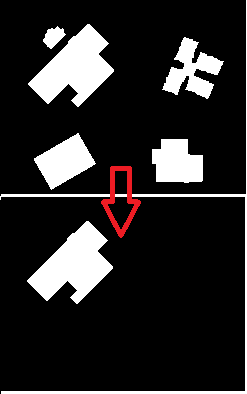
\includegraphics[scale=0.5]{figuras/componentes_conexos_extracao.png}
    \caption{Remoção dos N-1 menores componentes conexos, figura extraída e adaptada de https://docs.ufpr.br/~centeno/uni/pdi/exe/009/index.html}
    \label{fig:remocao_componentes_conexos}
\end{figure}

Na etapa 4 deste projeto, após a suavização de bordas, remoção de pequenas ilhas, e quebra de grandes componentes conexões como linha de separação da placa de estado, realizamos uma remoção dos N-7 menores componentes conexos que são de fato os caracteres de interesse a serem segmentados na imagem.

Ou seja, apenas os 7 maiores componentes conexos estarão presentes na imagem segmentada, partindo do princípio que as placas a serem analisadas neste projeto, tenham 7 caracteres, sendo 3 letras e 4 algarismos.

Este processo de ordenação, conforme já explicado anteriormente na seção de abertura, produziu resultados satisfatórios após a filtragem por abertura que quebrou grandes componentes conexos que não representavam caracteres.

Extração de bordas:
Gradiente interno:
A obtenção de um gradiente interno, é dada pela diferença entre uma imagem original e sua erosão através de um elemento estruturante. Como a imagem erodida tem dimensões menores do que a imagem original, o calculo dessa diferença irá produzir uma imagem contendo apenas a borda entre as 2 imagens.

O Gradiente Externo é um processo análogo ao interno, onde a imagem original passa por um processo de dilatação, e a diferença entre a imagem maior dilatada e a imagem original produz uma borda compreendida entre as 2 imagens.

O Gradiente Morfológico se dá pela diferença entre o gradiente interno e externo, todos os gradientes são ilustrados na Figura \ref{fig:tipos_gradientes}.

\begin{figure}[!ht]
    \centering
    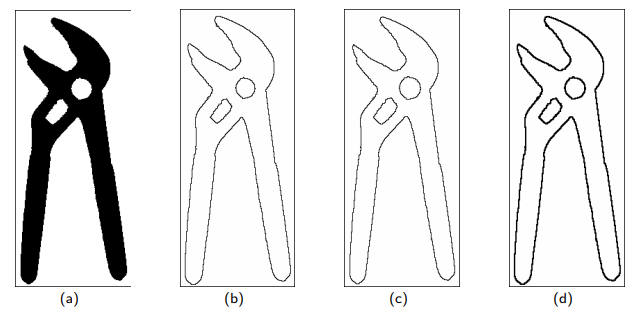
\includegraphics[scale=0.6]{figuras/gradientes.PNG}
    \caption{Tipos de Gradientes para detecção de bordas, imagem extraída de http://www.ic.unicamp.br/~helio/disciplinas/MO443/aula\_morfologia.pdf.}
    \label{fig:tipos_gradientes}
\end{figure}

\subsection{Descrição com código da cadeia}

%* Aqui podemos explicar que o projeto fornece o gradiente interno, externo e morfológico pode são usados para obtenção do código da cadeia, mas não reproduzi este experimento. Falar como se fosse uma etapa futura.

Ainda que além do escopo do projeto em questão, a aplicação dos gradientes morfológicos obtidos no passo anterior no algoritmo de código da cadeia (\textit{Chain code} \cite{freeman1961}) pode se apresentar como proposta futura para aprimorar a sistema de detecção desenvolvido neste trabalho. Portanto uma descrição de aplicação bem como a uma breve apresentação da teoria sobre código da cadeia é dada nesta secção.


Primeiramente, as imagens contendo apenas os elementos de borda são aplicadas no algoritmo de Código da Cadeia para a identificação dos caracteres presentes nas placas, Ao fim desta etapa obtém-se um conjunto de 7 caracteres alfa-numéricos equivalente ao padrão das placas brasileiras, sendo três letras e quatro números, no formato/sequência LLL-NNNN , sendo L letras e N números. 

O algoritmo de código da cadeia (do inglês, \textit{chain code}) foi proposto por \cite{freeman1961}. O princípio básico do algoritmo é codificar separadamente cada componente conectado na imagem, comumente chamados de "blobs". Para cada uma dessas regiões, um ponto no limite é selecionado e suas coordenadas são transmitidas. O codificador então se move ao longo do limite da região e, a cada passo, transmite um símbolo que representa a direção desse movimento. Isso continua até que o codificador retorne à posição inicial, momento em que o blob foi completamente descrito, e a codificação continua com o próximo blob da imagem.

\subsection{Avaliação da performance}

Na análise estatística da classificação binária, a métrica Dice (também conhecido com \textit{F1-score}) é uma medida da precisão de um teste. Ele considera a precisão p e o recall r do teste para calcular a pontuação: p é o número de resultados positivos corretos dividido pelo número de todos os resultados positivos retornados pelo classificador é o número de resultados positivos corretos dividido por o número de todas as amostras relevantes \cite{tustison2009}.

Similar ao método Dice, o índice de Jaccard, também conhecido como Intersecção sobre a União e o coeficiente de similaridade de Jaccard, é uma estatística usada para medir a semelhança e a diversidade dos conjuntos de amostras. O coeficiente de Jaccard mede a similaridade entre os conjuntos de amostras finitas e é definido como o tamanho da interseção dividido pelo tamanho da união dos conjuntos de amostras \cite{tustison2009}.
 
\chapter{Resultados e discussão}

\section{Resolução e tratamento de dimensões}
A Figura \ref{fig:placa_cinza} apresenta um exemplo de resultado da redução de dimensões, transformando assim a imagem em níveis de cinza.
É possível observar na figura \ref{fig:resolucao_pequena} a sensibilidade do processo à alteração da resolução e dimensionalidade das imagens de entradas dado que o algoritmo de segmentação trabalha com elementos estruturantes de tamanho pré-determinado. Ter uma imagem pequena, conforme já fundamento na seção sobre a operação de abertura, o elemento estruturante de tamanho pré-determinado poderá remover os caracteres menores de que n*B, sendo N a quantia de operações de abertura utilizadas neste algoritmo, e B o tamanho do elemento estruturante que neste caso foi escolhido N = 3, e B = 'square' de tamanho 5.\\


\begin{figure}[!ht]
    \centering
    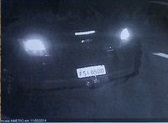
\includegraphics[scale=1]{resultados_finais/exemplo_placa_radar.jpg}
    \caption{Exemplo de imagem de radar de velocidade.}
    \label{fig:placa_radar}
\end{figure}

\begin{figure}[!ht]
    \centering
    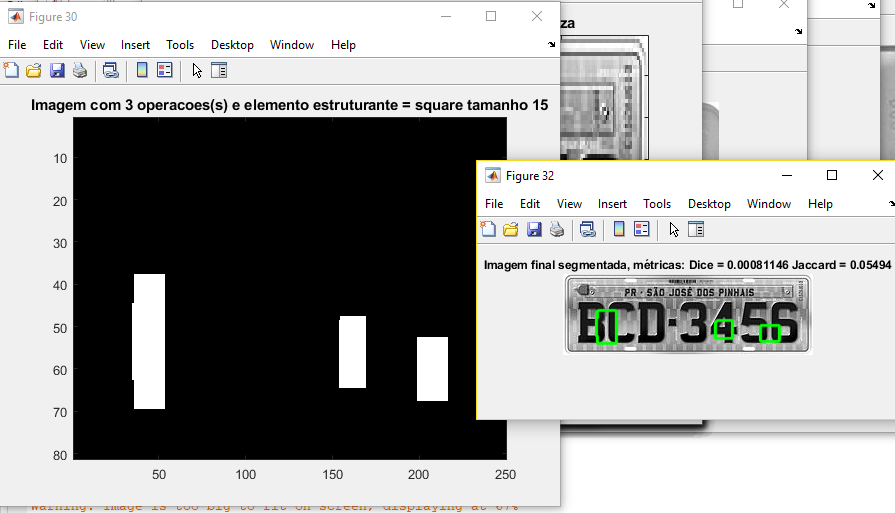
\includegraphics[scale=0.25]{dificuldades_experimentais/dimensionalidade.PNG}
    \caption{Segmentação falha de imagens pequenas.}
    \label{fig:resolucao_pequena}
\end{figure}

\begin{figure}[!ht]
    \centering
    \includegraphics[scale=0.3]{figuras/1.jpg}
    \caption{Exemplo de placa veicular com ruídos transformada para níveis de cinza.}
    \label{fig:placa_cinza}
\end{figure}

\section{Remoção de ruídos - Filtros}
A Figura \ref{fig:placa_medfilt} apresenta um exemplo de resultado da aplicação do filtro de mediana para a remoção de ruídos nas imagens das placas veiculares.

\begin{figure}[!ht]
    \centering
    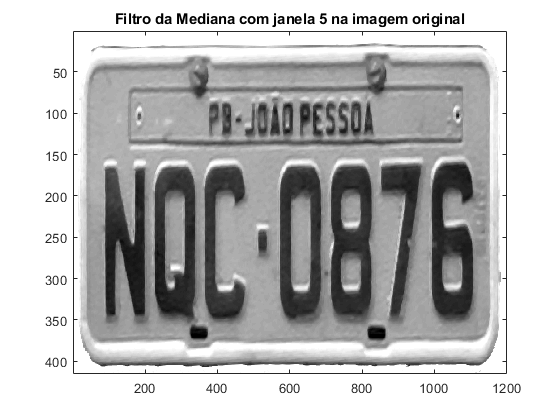
\includegraphics[scale=1]{figuras/1_filtro_med.png}
    \caption{Exemplo de placa veicular após a aplicação do filtro de mediana.}
    \label{fig:placa_medfilt}
\end{figure}

\section{Segmentação das imagens}

Os objetos a serem segmentados possuem intensidade predominantemente preta, ter um fundo preto na imagem atrapalha a aplicação do método de binarização por Otsu, produzindo a figura \ref{fig:cc_fundo_preto} tendo resultados finais conforme a figura \ref{fig:resultado_fundo_preto}, corrigindo o recorte para fundo branco a segmentação pode ser concluída com sucesso conforme a figura \ref{fig:resultado_fundo_branco}.

Imagens reais de câmeras de fiscalização ou estacionamento nos casos gerais são obtidas em escala de cinza para obtenção de imagens noturna, apesar da mesma estar em escala de cinza, a maior parte do ambiente estará com fundo preto, porém com a placa sempre destacada em uma posição fixa (dada que a câmera é fixa) da imagem, conforme Figura \ref{fig:placa_radar}. Logo técnicas de recorte e pré-processamento e pré-segmentação podem ser implementadas para obtenção da área da placa de interesse na segmentação.

\begin{figure}[!ht]
    \centering
    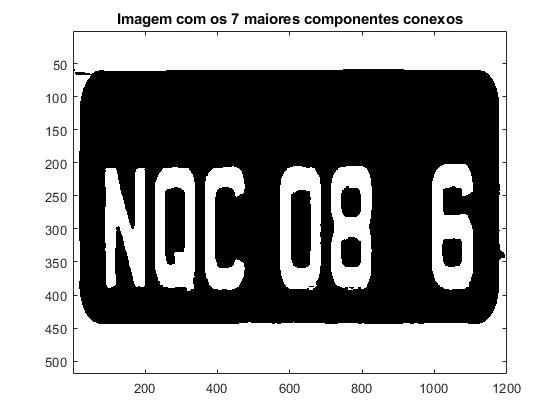
\includegraphics[scale=0.40]{dificuldades_experimentais/imagens_fundo_preto_2.jpg}
    \caption{Componentes conexos removidos erroneamente.}
    \label{fig:cc_fundo_preto}
\end{figure}

\begin{figure}[!ht]
    \centering
    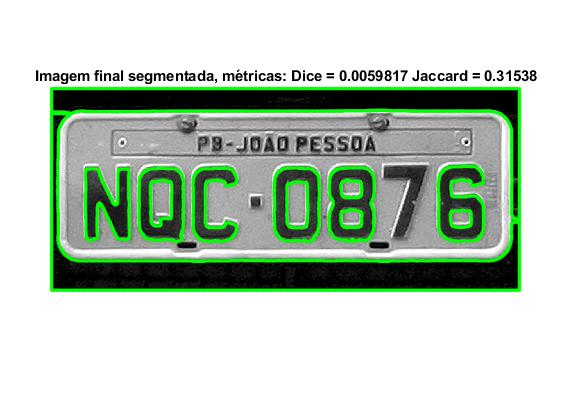
\includegraphics[scale=0.40]{dificuldades_experimentais/pre_processamento_fundo_preto.jpg}
    \caption{Resultado com fundo preto.}
    \label{fig:resultado_fundo_preto}
\end{figure}

\begin{figure}[!ht]
    \centering
    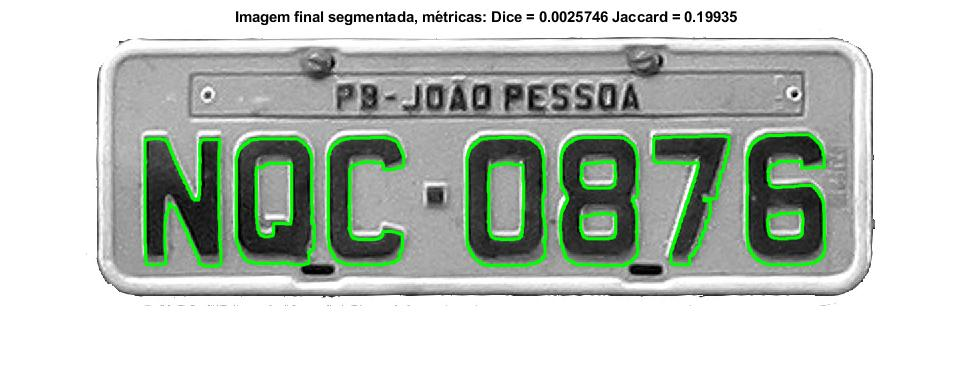
\includegraphics[scale=0.40]{dificuldades_experimentais/pre_processamento_fundo_branco.jpg}
    \caption{Resultado com fundo branco.}
    \label{fig:resultado_fundo_branco}
\end{figure}

A Figura \ref{fig:placa_segOtsu} apresenta a binarização por Otsu na Figura filtrada pela mediana.

\begin{figure}[!ht]
    \centering
    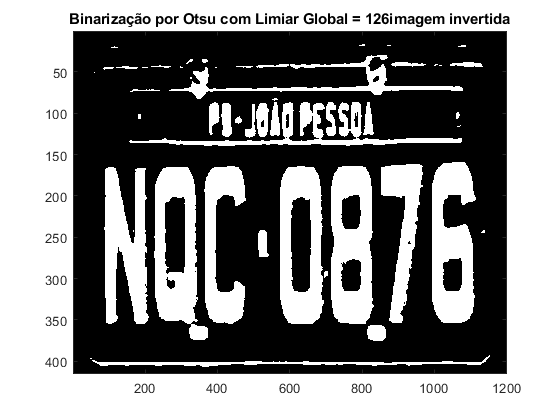
\includegraphics[scale=0.8]{figuras/1_bin.png}
    \caption{Exemplo de placa veicular após o processo de segmentação pela técnica de Otsu.}
    \label{fig:placa_segOtsu}
\end{figure}

\section{Filtragem de ruídos por operações morfológicas}

A partir da imagem segmentada neste projeto foi realizado o filtro de abertura, este filtro de abertura foi importante ao projeto, dado que o próximo filtro usado após a abertura, a remoção de componentes mantém apenas os N maiores componentes conexos da imagem, e traços de fundo conforme a Figura \ref{fig:placa_segOtsu} podem ser reconhecidos como um componente conexo maior do que o caractere da placa, e então este caractere é removido, pois sua ordem alterada na lista dos N maiores componentes conexos da imagem. Este fenômeno pode ser observado na Figura \ref{fig:cc_fundo_preto}.

A imagem utilizada de entrada (do inglês, \textit{input}) para o processo de filtragem por abertura é exemplificada pela Figura \ref{fig:abertura_depois}.
\begin{figure}[!ht]
    \centering
    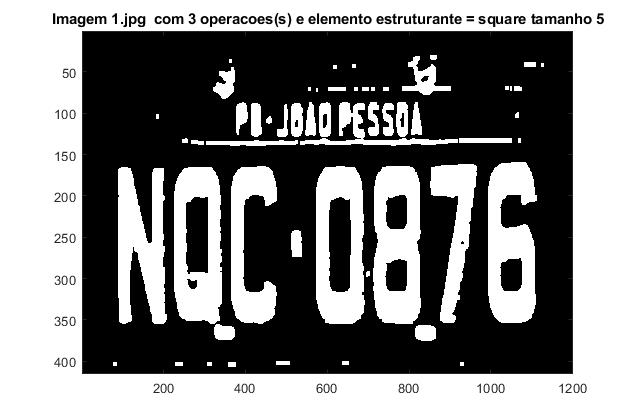
\includegraphics[scale=0.6]{etapas/etapa3.png}
    \caption{Imagem da 3a etapa do projeto, posterior ao processo de filtragem por abertura.}
    \label{fig:abertura_depois}
\end{figure}

A Figura \ref{fig:detalhe_sem_efeito_abertura} representa resultados obtidos sem o filtro da abertura, e a Figura \ref{fig:detalhe_efeito_abertura} são os resultados com o filtro. É possível observar suavização das linhas inferiores do caractere N, e também a correção do caractere Q que tinha seu traço inferior unido à sua forma principal.

\begin{figure}[!ht]
    \centering
    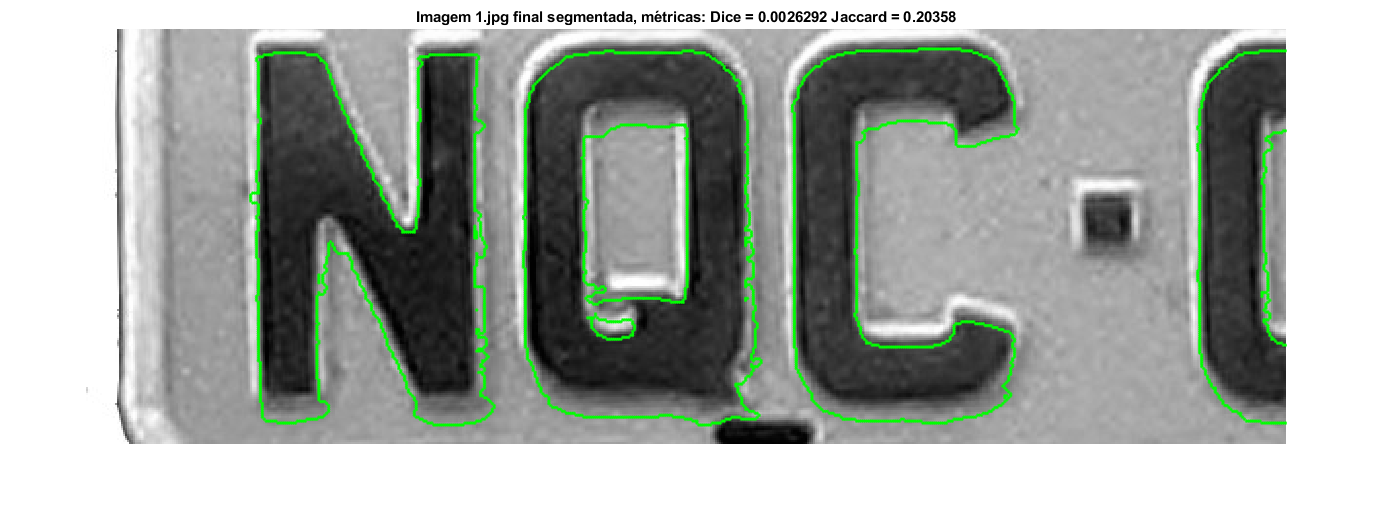
\includegraphics[scale=0.38]{etapas/detalhe_sem_efeito_abertura.png}
    \caption{Resultado final sem filtro de abertura.}
    \label{fig:detalhe_sem_efeito_abertura}
\end{figure}

\begin{figure}[!ht]
    \centering
    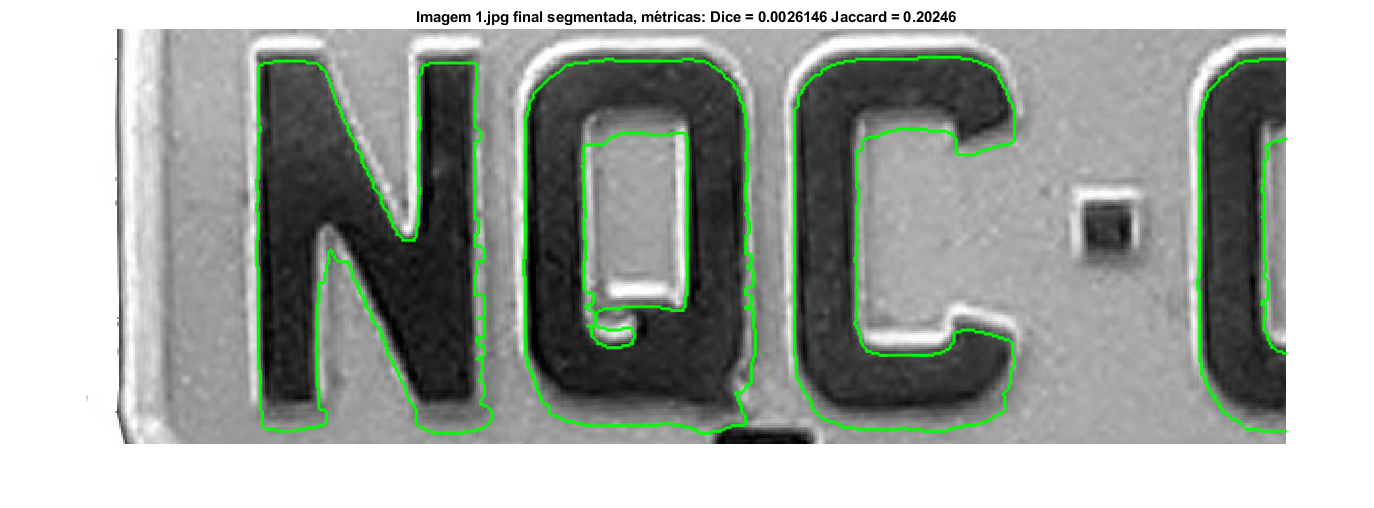
\includegraphics[scale=0.38]{etapas/detalhe_efeito_abertura.png}
    \caption{Resultado final com filtro de abertura.}
    \label{fig:detalhe_efeito_abertura}
\end{figure}

Por fim temos algumas Figuras abaixo (Figura \ref{fig:placa_0_segmentada},\ref{fig:placa_1_segmentada},\ref{fig:placa_4_segmentada},\ref{fig:placa_7_segmentada}) que representam o processo completo de segmentação.

\begin{figure}[!ht]
    \centering
    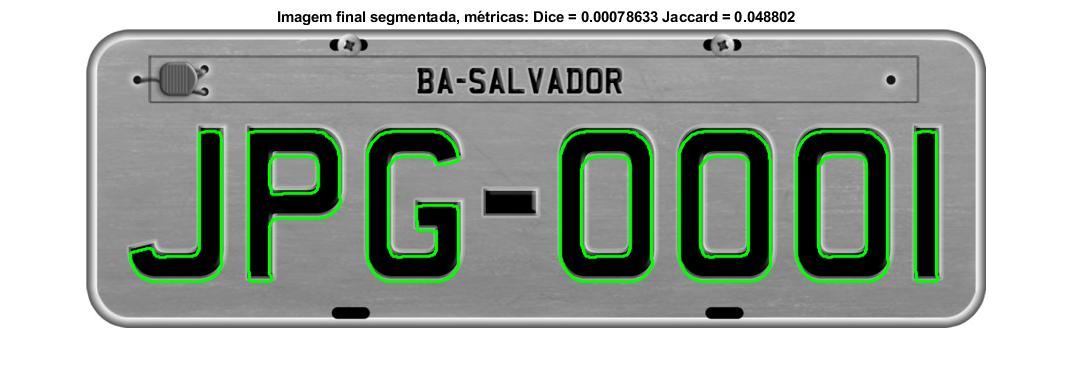
\includegraphics[scale=0.3]{resultados_finais/0.jpg}
    \caption{Placa Ideal Segmentada.}
    \label{fig:placa_0_segmentada}
\end{figure}

\begin{figure}[!ht]
    \centering
    \includegraphics[scale=0.45]{resultados_finais/1.jpg}
    \caption{Placa Real Segmentada.}
    \label{fig:placa_1_segmentada}
\end{figure}


\begin{figure}[!ht]
    \centering
    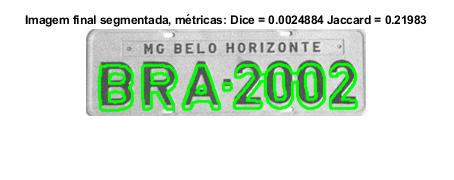
\includegraphics[scale=1]{resultados_finais/4.jpg}
    \caption{Placa Pequena Opaca Segmentada.}
    \label{fig:placa_4_segmentada}
\end{figure}

\begin{figure}[!ht]
    \centering
    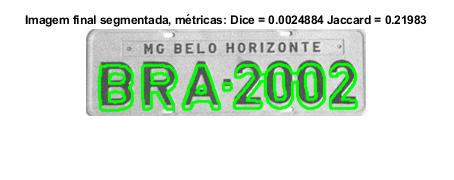
\includegraphics[scale=1]{resultados_finais/4.jpg}
    \caption{Placa Muito Pequena Segmentada.}
    \label{fig:placa_7_segmentada}
\end{figure}

\chapter{Conclusão}

Ao final dos experimentos realizados neste trabalho, podemos observar que as técnicas previstas como filtragem de ruído pelo método da mediana, binarização por Otsu, filtragem de ruído por operação morfológica de abertura e extração de borda por morfologia com gradientes, produzem resultados perceptíveis e satisfatórios para segmentar caracteres de uma placa veicular.

O procedimento em todas suas etapas de segmentação, depende de parametrizações específicas para determinados tipos de placas, e é sensível à alterações de resolução, pois são parametrizados tamanhos fixos de elementos estruturantes para remoção de ruídos bem como tamanhos fixos de janela de mediana. Ainda, é observado que o método também é sensível ao tipo de placa, pois na etapa de extração dos N maiores componentes conexos inferindo-se que os mesmos serão os caracteres de interesse das placas, o valor N é fixado como 7 dado o padrão atual de placas brasileiras que são 3 letras e 4 algarismos, logo se uma placa veicular conter uma quantia diferente de caracteres o processo de segmentação será falho.

Placas veiculares por serem uma identificação de um bem privado, são de difícil acesso para obtenção de bancos de imagens. Já que as mesmas podem sofrer processos de clonagem, espionagem, entre outros, bem como depender e autorização de uso de imagem.

O processo de segmentação que pode fornecer importantes descritores da imagem segmentada como por exemplo o código de freeman, aumentam muito a acurácia do processo de visão computacional e reconhecimento dos caracteres, em comparação se os mesmos fossem realizados sem o fornecimento de tais descritores.


\postextual

%\nocite{microbiologia}
%\nocite{hemibiotrophiccacao}
%\nocite{involvement}
%\nocite{productionoflytic}
%\nocite{causafungo}
%\nocite{elementosestrategia}
%\nocite{futuroagrobiotec}
%\nocite{epivassou}
%\nocite{princdoen}
%\nocite{kilaru}
%\nocite{grif}

% ----------------------------------------------------------
% Referências bibliográficas
% ----------------------------------------------------------
\bibliography{referencias} 

\end{document}
